% Options for packages loaded elsewhere
\PassOptionsToPackage{unicode,pdfpagelabels}{hyperref}
\PassOptionsToPackage{hyphens}{url}
\PassOptionsToPackage{dvipsnames,svgnames,x11names}{xcolor}
%
\documentclass[
  12pt,
  a4paper,
]{report}

\usepackage{amsmath,amssymb}
\usepackage{iftex}
\ifPDFTeX
  \usepackage[T1]{fontenc}
  \usepackage[utf8]{inputenc}
  \usepackage{textcomp} % provide euro and other symbols
\else % if luatex or xetex
  \usepackage{unicode-math}
  \defaultfontfeatures{Scale=MatchLowercase}
  \defaultfontfeatures[\rmfamily]{Ligatures=TeX,Scale=1}
\fi
\usepackage{lmodern}
\ifPDFTeX\else  
    % xetex/luatex font selection
\fi
% Use upquote if available, for straight quotes in verbatim environments
\IfFileExists{upquote.sty}{\usepackage{upquote}}{}
\IfFileExists{microtype.sty}{% use microtype if available
  \usepackage[]{microtype}
  \UseMicrotypeSet[protrusion]{basicmath} % disable protrusion for tt fonts
}{}
\makeatletter
\@ifundefined{KOMAClassName}{% if non-KOMA class
  \IfFileExists{parskip.sty}{%
    \usepackage{parskip}
  }{% else
    \setlength{\parindent}{0pt}
    \setlength{\parskip}{6pt plus 2pt minus 1pt}}
}{% if KOMA class
  \KOMAoptions{parskip=half}}
\makeatother
\usepackage{xcolor}
\usepackage[top=2cm,bottom=2cm,left=1.5cm,right=1.5cm,marginparsep=2cm]{geometry}
\setlength{\emergencystretch}{3em} % prevent overfull lines
\setcounter{secnumdepth}{5}
% Make \paragraph and \subparagraph free-standing
\makeatletter
\ifx\paragraph\undefined\else
  \let\oldparagraph\paragraph
  \renewcommand{\paragraph}{
    \@ifstar
      \xxxParagraphStar
      \xxxParagraphNoStar
  }
  \newcommand{\xxxParagraphStar}[1]{\oldparagraph*{#1}\mbox{}}
  \newcommand{\xxxParagraphNoStar}[1]{\oldparagraph{#1}\mbox{}}
\fi
\ifx\subparagraph\undefined\else
  \let\oldsubparagraph\subparagraph
  \renewcommand{\subparagraph}{
    \@ifstar
      \xxxSubParagraphStar
      \xxxSubParagraphNoStar
  }
  \newcommand{\xxxSubParagraphStar}[1]{\oldsubparagraph*{#1}\mbox{}}
  \newcommand{\xxxSubParagraphNoStar}[1]{\oldsubparagraph{#1}\mbox{}}
\fi
\makeatother


\providecommand{\tightlist}{%
  \setlength{\itemsep}{0pt}\setlength{\parskip}{0pt}}\usepackage{longtable,booktabs,array}
\usepackage{calc} % for calculating minipage widths
% Correct order of tables after \paragraph or \subparagraph
\usepackage{etoolbox}
\makeatletter
\patchcmd\longtable{\par}{\if@noskipsec\mbox{}\fi\par}{}{}
\makeatother
% Allow footnotes in longtable head/foot
\IfFileExists{footnotehyper.sty}{\usepackage{footnotehyper}}{\usepackage{footnote}}
\makesavenoteenv{longtable}
\usepackage{graphicx}
\makeatletter
\def\maxwidth{\ifdim\Gin@nat@width>\linewidth\linewidth\else\Gin@nat@width\fi}
\def\maxheight{\ifdim\Gin@nat@height>\textheight\textheight\else\Gin@nat@height\fi}
\makeatother
% Scale images if necessary, so that they will not overflow the page
% margins by default, and it is still possible to overwrite the defaults
% using explicit options in \includegraphics[width, height, ...]{}
\setkeys{Gin}{width=\maxwidth,height=\maxheight,keepaspectratio}
% Set default figure placement to htbp
\makeatletter
\def\fps@figure{htbp}
\makeatother

\usepackage{graphicx}
\usepackage{tcolorbox}
\usepackage{siunitx}
\usepackage{xcolor}
\usepackage{titlesec}
\usepackage{float}
\sisetup{per-mode = symbol} % Set SI unit fractions to use a solidus
\definecolor{boxheadcol}{HTML}{D6D6F0} % #D6D6F0
\definecolor{boxbodycol}{HTML}{EBEBF7} % #EBEBF7
\definecolor{boxtitlecol}{HTML}{4A45B4} % #4A45B4
\tcbset{title filled}
\titlespacing*{\chapter}{0pt}{-20pt}{10pt}
\titlespacing*{\part}{0pt}{20pt}{10pt}
\titlespacing*{\section}{0pt}{20pt}{10pt}
\makeatletter
\@ifpackageloaded{bookmark}{}{\usepackage{bookmark}}
\makeatother
\makeatletter
\@ifpackageloaded{caption}{}{\usepackage{caption}}
\AtBeginDocument{%
\ifdefined\contentsname
  \renewcommand*\contentsname{Table of contents}
\else
  \newcommand\contentsname{Table of contents}
\fi
\ifdefined\listfigurename
  \renewcommand*\listfigurename{List of Figures}
\else
  \newcommand\listfigurename{List of Figures}
\fi
\ifdefined\listtablename
  \renewcommand*\listtablename{List of Tables}
\else
  \newcommand\listtablename{List of Tables}
\fi
\ifdefined\figurename
  \renewcommand*\figurename{Figure}
\else
  \newcommand\figurename{Figure}
\fi
\ifdefined\tablename
  \renewcommand*\tablename{Table}
\else
  \newcommand\tablename{Table}
\fi
}
\@ifpackageloaded{float}{}{\usepackage{float}}
\floatstyle{ruled}
\@ifundefined{c@chapter}{\newfloat{codelisting}{h}{lop}}{\newfloat{codelisting}{h}{lop}[chapter]}
\floatname{codelisting}{Listing}
\newcommand*\listoflistings{\listof{codelisting}{List of Listings}}
\makeatother
\makeatletter
\makeatother
\makeatletter
\@ifpackageloaded{caption}{}{\usepackage{caption}}
\@ifpackageloaded{subcaption}{}{\usepackage{subcaption}}
\makeatother

\ifLuaTeX
  \usepackage{selnolig}  % disable illegal ligatures
\fi
\usepackage{bookmark}

\IfFileExists{xurl.sty}{\usepackage{xurl}}{} % add URL line breaks if available
\urlstyle{same} % disable monospaced font for URLs
\hypersetup{
  pdftitle={COMPSYS 304: Computer Architecture},
  pdfauthor={Nicholas Russell},
  colorlinks=true,
  linkcolor={blue},
  filecolor={Maroon},
  citecolor={Blue},
  urlcolor={Blue},
  pdfcreator={LaTeX via pandoc}}


\title{COMPSYS 304: Computer Architecture}
\usepackage{etoolbox}
\makeatletter
\providecommand{\subtitle}[1]{% add subtitle to \maketitle
  \apptocmd{\@title}{\par {\large #1 \par}}{}{}
}
\makeatother
\subtitle{Lecture Notes}
\author{Nicholas Russell}
\date{2024-03-09}

\begin{document}
\maketitle

\renewcommand*\contentsname{Table of contents}
{
\hypersetup{linkcolor=}
\setcounter{tocdepth}{2}
\tableofcontents
}

\bookmarksetup{startatroot}

\chapter*{Introduction}\label{introduction}
\addcontentsline{toc}{chapter}{Introduction}

\markboth{Introduction}{Introduction}

These notes are compiled from the lectures of COMPSYS 304. They are
intended as a personal reference to help with assignments, exam
preparation, and understanding key concepts in Computer Architecture.

The notes are organised by lecture and cover a wide range of topics from
basic computer architecture principles to more advanced subjects like
MIPS implementation and performance analysis. Feel free to add personal
insights, additional readings, or questions as you review this material.

\section*{Organisation of the Notes}\label{organisation-of-the-notes}
\addcontentsline{toc}{section}{Organisation of the Notes}

\markright{Organisation of the Notes}

The notes are divided by lecture content, with each section
corresponding to a specific set of topics. Here's how they're organized:

\begin{itemize}
\item
  \textbf{Lecture 1-3: Basics of Computer Architecture}\\
  Key topics include Instruction Set Architecture (ISA), memory
  hierarchy, and basic CPU organisation.
\item
  \textbf{Lecture 4-6: MIPS Architecture}\\
  Covers the MIPS instruction set, control flow, and subroutine
  handling.
\item
  \textbf{Lecture 7-9: CPU Implementation}\\
  Focuses on different methods for implementing CPUs and the trade-offs
  involved.
\item
  \textbf{Lecture 10-12: Digital Circuits and Datapath Design}\\
  Reviews fundamental digital circuit concepts and discusses the design
  of a MIPS datapath.
\item
  \textbf{Lecture 13-15: Performance Analysis}\\
  Provides an in-depth look at how different design choices impact CPU
  performance.
\end{itemize}

\section*{How I Use These Notes}\label{how-i-use-these-notes}
\addcontentsline{toc}{section}{How I Use These Notes}

\markright{How I Use These Notes}

These notes are a living document, and I intend to update them as I gain
a deeper understanding of the material. Here's how I use them:

\begin{itemize}
\tightlist
\item
  \textbf{Quick Reference}: For quick lookups, the Table of Contents
  will help me jump directly to the relevant section.
\item
  \textbf{In-Depth Study}: For exam preparation, I'll revisit each
  section, ensuring I understand each concept before moving on.
\item
  \textbf{Personal Insights}: I'll be adding my own thoughts, additional
  notes from readings, and potential questions for further study.
\end{itemize}

I might also include exercises or practical examples that help solidify
my understanding of the more complex topics.

\part{Lectures 1 - 3}

\chapter{Introduction \& Course
Overview}\label{introduction-course-overview}

This chapter provides an introduction to the course, some background,
and an overview of the course itself.

\section{Background}\label{background}

In the last six decades, computer technology has made incredible
progress due to innovations in both \textbf{semiconductor technology}
and computer \textbf{architecture}.

\subsection{\texorpdfstring{What do we mean from
\emph{Performance}?}{What do we mean from Performance?}}\label{what-do-we-mean-from-performance}

The relative performance can be measured by standard benchmarks, which
depend on the specific target applications.

\textbf{\emph{Performance depends on clock frequency and other factors,
as discussed more in later chapters.}}

\subsection{Intel X86 Processor from 1978 to
2018:}\label{intel-x86-processor-from-1978-to-2018}

\begin{itemize}
\item
  \textbf{Intel 8086} - (1978): 1 core, 1 W, 5 - 10 MHz
\item
  \textbf{Core i7-8086K} - (2018): 6 cores, 95 W, 4 GHz
\end{itemize}

\section{Course Details}\label{course-details}

\subsection{Learning outcomes}\label{learning-outcomes}

The main learning outcomes of this course are:

\begin{itemize}
\item
  \textbf{To understand the basics of modern computer architectures and
  quantitative principles of computer design in order to develop a
  conceptual understanding of issues involved in designing a high
  performance computer system.}
\item
  \textbf{To use and apply this knowledge to design computer systems or
  select computers for specific tasks. This course will give you an
  understanding of the effects of design decisions on system performance
  and makes you a well-informed consumer in addition to a processor
  designer.}
\end{itemize}

Recommended Textbook:

\begin{itemize}
\item
  David A. Patterson and John L. Hennessey, Computer Organization and
  Design: The Hardware/Software Interface, Fifth edition, 2013 by
  Elsevier/Morgan Kaufmann Publishers (or 3rd or 4th editions).
\item
  Lecture notes provided on canvas (these will be summarised in these
  notes).
\end{itemize}

\subsection{Course Overview (learning
outcomes)}\label{course-overview-learning-outcomes}

\textbf{Part 1:} \emph{In this part you will learn to:}

\begin{itemize}
\item
  Design and evaluate the instruction set architectures (both RISC and
  CISC) and how it can be related to the hardware/software interface in
  a computer system with a quick review of assembly programming.
\item
  Understand different processor implementation methods including the
  basic single-cycle implementation and how it can be extended to a
  multi-cycle, pipelined and superscalar implementations.
\item
  Understand performance evaluation techniques and their relation to the
  target applications and the processor workload.
\end{itemize}

\textbf{Part 2:} \emph{In this part you will learn to:}

\begin{itemize}
\item
  Understand the memory hierarchy in a modern computer system and its
  impact on the performance of the system. This includes physical and
  virtual memory systems and basics of cache memories.
\item
  Understand some basic principles of parallel computing using special
  topics in this course (more advanced materials covered in some
  elective courses).
\end{itemize}

\subsection{Assessment}\label{assessment}

Three assignments and one test in addition to the final exam. The first
assignment is mainly on the instruction set architecture design,
hardware/software interfacing and review of assembly programming. The
second assignment is related to processor implementation and performance
issues. The third assignment is related to memory hierarchy system and
multiprocessing.

\textbf{The test only covers the first part of the course. The final
exam covers the whole course.}

\begin{itemize}
\item
  \textbf{Assignment 1: 8\% due Fri. 9 August.}
\item
  \textbf{Assignment 2: 7\% due Fri. 23 August.}
\item
  \textbf{Assignment 3: 15\% due Fri. 4 October.}
\item
  \textbf{Test: 20\% (in week 7, Wednesday 11 September)}
\item
  \textbf{Final exam: 50\%}
\end{itemize}

\chapter{Basics of Computer
Architecture}\label{basics-of-computer-architecture}

This chapter begins the journey into the content of this course.

\section{What is Computer
Architecture?}\label{what-is-computer-architecture}

\begin{itemize}
\item
  \textbf{ISA:} The programmer-visible instructions --- ISA serves as
  the boundary between the hardware and software.
\item
  \textbf{Organization:} high-level aspects of computer design (e.g.~the
  internal design of the CPU, the memory system, the interconnection
  structure, \ldots)
\item
  \textbf{Hardware:} detailed logic design, circuit-level design,
  packaging technology, etc.
\end{itemize}

\section{Review: Memory Organization}\label{review-memory-organization}

\begin{itemize}
\item
  Memory is viewed as a large, one-dimensional array, which has an
  address range.
\item
  A memory address is an index into the array
\item
  The index usually points to a byte of memory.
\item
  To access a larger word (e.g., a 32-bit word or 4 bytes), four
  consecutive memory locations are accessed.
\end{itemize}

\emph{Memory access time} is the amount of time required to read
(usually one byte) or write data (usually one byte) from/to memory.

\section{An Overview of Memory Speed vs.~CPU
Speed}\label{an-overview-of-memory-speed-vs.-cpu-speed}

The rate of memory speed increase has been less than processors speed
increase

Fast memory is more expensive per bit than slow memory, so a
\textbf{memory hierarchy} is often used to give a performance close to
the fastest memory with a lower average cost per bit.

\section{Processor and Memory
Hierarchy}\label{processor-and-memory-hierarchy}

\begin{figure}[H]

\begin{minipage}{0.40\linewidth}
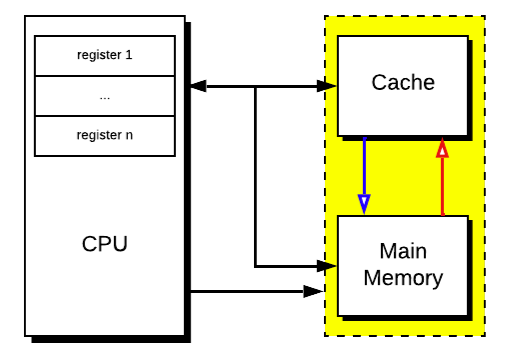
\includegraphics{lecture1-3/images/processorhierarchy.png}\end{minipage}%
%
\begin{minipage}{0.60\linewidth}

\begin{tcolorbox}[colback=boxbodycol, colframe=boxheadcol, colbacktitle=boxheadcol, title=\textcolor{red}{\emph{Processor Registers: }}\textcolor{blue}{The smallest and fastest memory for CPU.}]
Typically, 32 to 64 registers, each of them may be 32 or 64 bits with
typical access time of \textcolor{blue}{\emph{nanoseconds or less}}

\end{tcolorbox}

\begin{tcolorbox}[colback=boxbodycol, colframe=boxheadcol, colbacktitle=boxheadcol, title=\textcolor{red}{\emph{Cache Memory: }}\textcolor{blue}{Slower than registers.}]
Typically 8 to 256 Kbytes with an access time about a
\textcolor{blue}{\emph{few nanoseconds or less}}

\end{tcolorbox}

\begin{tcolorbox}[colback=boxbodycol, colframe=boxheadcol, colbacktitle=boxheadcol, title=\textcolor{red}{\emph{Main Memory: }}\textcolor{blue}{Slower than cache memory.}]
Hundreds of Mega bytes with an access time about
\textcolor{blue}{\emph{tens of nanoseconds}}

\end{tcolorbox}

\end{minipage}%

\end{figure}%

\section{Example of Intel Processors}\label{example-of-intel-processors}

\begin{figure}[H]

\begin{minipage}{0.50\linewidth}

\begin{tcolorbox}[colback=boxbodycol, colframe=boxheadcol, colbacktitle=boxheadcol, title=\textcolor{red}{\emph{Pentium Processor Architecture (simplified) }}]
An example of architectural innovations made by processor designers (to
improve computer systems performance) \textcolor{red}{(Source: Intel)}

\end{tcolorbox}

\end{minipage}%
%
\begin{minipage}{0.50\linewidth}
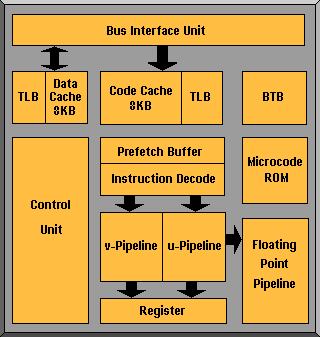
\includegraphics[width=8cm,height=\textheight]{lecture1-3/images/22pentium.png}\end{minipage}%
\newline
\begin{minipage}{0.50\linewidth}

\begin{tcolorbox}[colback=boxbodycol, colframe=boxheadcol, colbacktitle=boxheadcol, title=\textcolor{red}{\emph{Intel Core i7}}]
The Core i7 die and major components. (more than 700 million transistors
in a die with area \qty{263}{\mm\squared} in \qty{45}{\nm} technology).
\textcolor{red}{(Source: Intel)}

\end{tcolorbox}

\end{minipage}%
%
\begin{minipage}{0.50\linewidth}
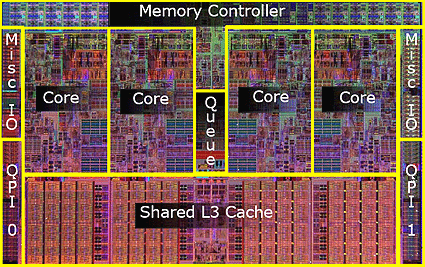
\includegraphics[width=8cm,height=\textheight]{lecture1-3/images/corei7diagram.png}\end{minipage}%

\end{figure}%

\chapter{Instruction set Architecture
(ISA)}\label{instruction-set-architecture-isa}

ISA is the interface between hardware and low-level software

\begin{tcolorbox}[colback=boxbodycol, colframe=boxheadcol, title=Some modern instruction set architectures:, coltitle=boxtitlecol, colbacktitle=boxheadcol]
\textcolor{red}{\textbf{80x86}}, Itanium, PowerPC,
\textcolor{red}{\textbf{MIPS}}, SPARC, HP,
\textcolor{red}{\textbf{ARM}}, \textcolor{red}{\textbf{RISC-V}}

\end{tcolorbox}




\end{document}
